%--------------------------------------------------------------------------------
\documentclass[]{YIC2015}

% --------------------------------------------------------------------------------
% Include here your latex packages
%--------------------------------------------------------------------------------
\usepackage{graphicx}
\usepackage{color}
\usepackage{url}

% --------------------------------------------------------------------------------
% Article's title, with capital letter only at the beginning
%--------------------------------------------------------------------------------
\title{Modeling the I/O behavior of the NEST simulator using a proxy}

% -------------------------------------------------------------------------------
% List of authors
% --------------------------------------------------------------------------------
% Put the initials and surname of the first author ('et al.' if applicable) in
% square brackets before the command \author
%
% Identify the corresponding author with the command \corref and each author
% with the command \authref{a,b,...} according to the affiliation
%
\author[T. Schumann et al.]{%
  T. Schumann\authref{a}\corref,
  W. Frings\authref{b},
  A. Peyser\authref{c},
  W. Schenck\authref{c},
  K. Thust\authref{b},
  S. L\"uhrs\authref{b},
  J.M. Eppler\authref{c}
}

% --------------------------------------------------------------------------------
% Affiliations
% --------------------------------------------------------------------------------
\address{\authaddr{a}{Institute of Neuroscience and Medicine (INM-6), Computational and Systems Neuroscience \\ %
    Institute for Advanced Simulation (IAS-6) \\ %
    J\"ulich Aachen Research Alliance \\ %
    Forschungszentrum J\"ulich GmbH \\ %
    52425 J\"ulich, Germany}
  \authaddr{b}{J\"ulich Supercomputing Centre \\ %
    Institute for Advanced Simulation \\ %
    Forschungszentrum J\"ulich GmbH\\ %
    52425 J\"ulich, Germany}
  \authaddr{c}{Simulation Lab Neuroscience - Bernstein Facility for Simulation and Database Technology \\ %
    Institute for Advanced Simulation \\ %
    J\"ulich Aachen Research Alliance \\ %
    Forschungszentrum J\"ulich GmbH \\ %
    52425 J\"ulich, Germany}
}
%
% --------------------------------------------------------------------------------
% Email address of the corresponding author
% --------------------------------------------------------------------------------
\corauth{till.schumann@rwth-aachen.de}

% --------------------------------------------------------------------------------
% Abstract
% --------------------------------------------------------------------------------
\abstract{\textit{ NEST \cite{NEST} is a simulator for spiking neural
    networks. It runs on ordinary desktop computers and notebooks,
    small clusters and supercomputers \cite{Plesser07}. Storing
    simulation data efficiently is essential for neuroscientific
    studies but not trivial on supercomputers with centralized
    storage. To assess different I/O strategies and libraries, we have
    implemented a \emph{proxy} which imitates the writing behavior of
    NEST. This proxy allows benchmarking and statistical analysis, and
    thus consequent optimizations, without the complexity of running
    full NEST simulations.}}

% --------------------------------------------------------------------------------
% Keywords - must be separated by semicolon and no capital letters.
% --------------------------------------------------------------------------------
\keywords{parallel I/O; simulation; neuronal networks; supercomputer;
  threading; MPI}

% --------------------------------------------------------------------------------
% Beginning of document
% --------------------------------------------------------------------------------
\begin{document}

\maketitle

% --------------------------------------------------------------------------------
% Beginning of one section
% --------------------------------------------------------------------------------
\section{Introduction}
%
Over the past 20 years, the NEST Initiative \cite{NESTInitiative} has
developed the NEST \cite{NEST} simulator for spiking neural network
models. It is used in computational neuroscience to simulate the
dynamics of the interaction between nerve cells. The systems explored
with NEST range from small networks simulated on local machines up to
large brain-scale circuits using the full capabilities of the world's
leading supercomputers. To have this flexibility, NEST is parallelized
in a hybrid fashion using threads on a compute node and MPI to
communicate between the compute nodes \cite{Plesser07}.  Storing
simulation data from such a massively parallel application efficiently
during runtime is essential for neuroscientific studies, but not a
trivial task on a supercomputer with centralized storage.

Virtual recording devices store neuronal properties such as spiking
activity and membrane voltage to disk. With increasing numbers of
devices and compute nodes, opening files and writing to them becomes a
major bottleneck, thus requiring new I/O strategies.

Until now, NEST has used the C++ standard I/O library to store
simulation results to disk. In the case of large scale simulations on
supercomputers, a huge number of virtual devices can request file
access simultaneously, leading to write system calls becoming a
significant element of overhead. We have therefore investigated
possible performance gains by replacing the current I/O paradigm with
calls to parallelized I/O libraries which could avoid serialization
bottlenecks when interacting with underlying file systems such as GPFS
\cite{GPFS} for highly parallel simulations.

\section{Requirements for the I/O interface}

NEST is used for a large variety of use cases, each having different
requirements on efficiency and output file formats. To make the I/O of
NEST more flexible, an interface wass developed which connects the
virtual devices with the I/O libraries. Taking into account that some
of the libraries use parallel I/O, the interface contains
synchronization functions besides the usual open, close and write
functions. These synchronization function allows inter-node
communication during the simulation to guarantee that the write
function is called simultaneously on all nodes.

\begin{figure}[htbp]
\centering %
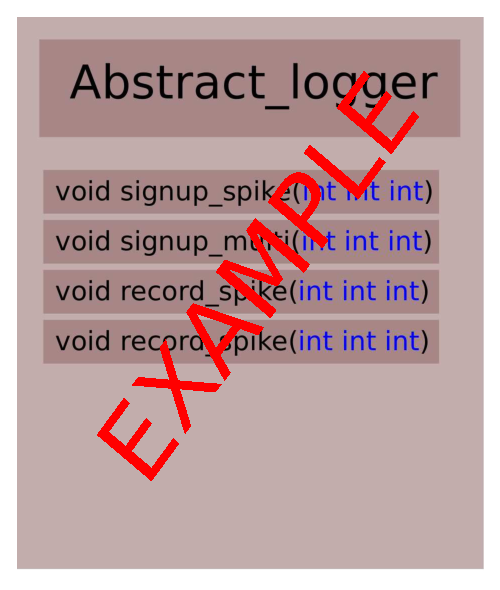
\includegraphics[scale=0.5]{loggerinterface.eps}
\caption{ILogger is the implemented I/O interface for the virtual recording devices. 
Three differenct logger interfaces are available: \emph{ASCIILogger} (see section \ref{sec:ascii}),
\emph{SIONLogger} (see section \ref{sec:sionlib}) and \emph{HDF5Logger} (see section \ref{sec:hdf5})}
\label{fig:loggerinterface}
\end{figure}

\subsection{Use cases of NEST}

\pleasewrite{Jochen}{the random balanced network and the reduced model of the visual
cortex}
\begin{itemize}
  \item{Random balanced network: Dry-run simulation for M=32, T=16, N=300,000, mean firing frequ. of 7 Hz}
  \item{Microcircuit model: Real simulation of only one area, run over 1000.0 ms: \\
- Number of MPI processes: 32\\
- Number of threads per MPI process: 8\\
- Number of virtual processes (VPs): 256 (32x8)\\
- Number of spike detectors per VP: 8\\
- Number of neurons attached to each spike detector: 10000/256 (ca.)\\
- Number of multimeters per VP: 8\\
- Number of neurons attached to each multimeter: 500/256\\
- MinDelay interval: Most likely equal to h step (= 0.1 ms)\\
- Overall number of neurons in the network: 80,000}
\end{itemize}

\section{An I/O proxy to ease development}

To develop new I/O strategies, information about the writing behavior
of NEST is necessary. In order to get this information, the main
algorithms of NEST were analyzed and typical writing behavior was
estimated.

Given that NEST is a neuronal simulator, which simulates an arbitrary
neuronal network based on the rules given in a simulation script, the
program structure only gives approximate and not exact information
about the writing behavior. To get the real runtime behavior, the code
analysis was acompanied by runtime measurements which covers standard
use cases.

\subsection{Analysis of NEST code}

% The algorithms of NEST are globally time-driven with constant time
% steps. In each time step all neurons are updated iteratively.

The main program structure of NEST can be reduced to an iteration loop
of gather, scatter and update functions of the network. Gather and
Scatter calls distribute the node states in the network. The update
function calls for each node internal algorithms, which process the
incoming information and update their state.

If the network node is a virtual recording device, it calls writing
functions depending on the incoming information. There are two types
of virtual recording devices: \emph{Spikedetectors} handling spike
events and \emph{Multimeters} requesting internal parameters of node
objects.

Whether a writing call occurs depends on the neuronal network
structure and activity. Statistical values are used to reproduce the
quasi-random occurrence of writing calls in the update functions.

\subsection{Measurements of runtime behavior}

To generate reliable timing measurements of the runtime behavior, part
of the NEST code was manually instrumented with Score--P \cite{ScoreP}
--- especially the relevant member functions of the virtual recording
devices and within them the calls to lower--level I/O functions.

We used the instrumented NEST binary to generate trace data for the
two use cases described above. From the trace data, we derived several
statistical measures which describe the runtime behavior of NEST,
e.g.~the distribution of onsets of spike writing in each thread
relative to the start of the update phase in the main simulation cycle
of NEST.

\subsection{Working principle of NESTProxy}

The NESTProxy contains three main parts: Construction of the network,
iteration loop and destruction of the network.

In the first part each node creates a set of \emph{Spikedetector} and
\emph{Multimeter} objects.  The number is taken from the input
parameters \emph{numberOfSpikeDetectorsPerThread} and
\emph{numberOfMultimetersPerThread} respectivly.

The objects are initialized with their parameters (see Table
\ref{tab:table-silva1}) (for \emph{Spikedetector}:
\emph{spikesPerDetector} and \emph{Multimeter}:
\emph{samplingIntervalsOfMeter}, \emph{numberOfValuesWrittenByMeter}.

The iteration loops contains a sleep function, which uses the
distribution from \emph{deadTimeDeliver}, all update function calls of
the recording device object and between this calls a sleep function,
which uses the distribution from \emph{deadTimeUpdate}.

During the update function each \emph{Spikedetector} or
\emph{Multimeter} object calls one or multiple write functions,
depending on its distribution variable.

%The random implementation is based on the \emph{C++11} standard library.
\begin{table}[htdp]
\caption{Stochastical parameters, which are input parameters of the NESTProxy}
\centering
\begin{tabular}{lll}
\hline\hline
\textbf{Type} & \textbf{Name}                   & \textbf{Description} \\ \hline
Integer       & numberOfSpikeDetectorsPerThread & number of SpikeDetectors per thread  \\
Integer       & numberOfMultimetersPerThread    & number of Multimeters per thread  \\
Distribution  & spikesPerDetector               & number of spikes generated at each \\
	      &					& SpikeDetector per iteration  \\
Distribution  & samplingIntervalsOfMeter        & sampling interval of the Multimeters  \\
Distribution  & numberOfValuesWrittenByMeter    & number of written values by each \\
	      &					& Multimeter in sampling interval  \\
Distribution  & deadTimeUpdate                  & sleeping timings between SpikeDetector \\
	      &					& and Multimeters writing operations \\
Distribution  & deadTimeDeliver                 & sleeping time in deliver function  \\
\hline\hline
\end{tabular}
\label{tab:table-silva1}
\caption{Input parameters of the NESTProxy. Following distributions
are implemented: Standard, Poisson, Binominal and fixed values}
\end{table}

\section{Implement drivers}
Based on the interface described above different drivers are
implemented.

\subsection{ASCII}
\label{sec:ascii}
Current versions of NEST use the standard C++ I/O stream library
\cite{stream} to permanently store results as plain text files
containing information as time stamps as floating point strings. The
advantage of such a scheme is simplicity in implementation and in
post-processing for analysis tools in addition to plain-text's
self-descriptive nature.

However for large-scale simulations, this leads to: 1) excessively
large amounts of data written to disk which is both a performance
issue and a practical storage problem; 2) a serialization bottleneck
when opening a separate file per virtual recording device; and 3) a serialization
bottleneck for metadata updates in the file system when new blocks are
allocated.
\pleasewrite{Alex}{The ASCII driver has for each virtual recording device a file. The virtual recording devices live on the task.}

One solution used in recent releases of NEST has been the global spike
detector \cite{gsd}: a single file is opened by a dedicated rank to
store spiking events, a low cost solution since currently all ranks
see all spike events through MPI collective communication.

On the other hand, such an approach has several long-term
consequences: 1) it constitutes a serialization bottleneck as spike
event I/O is handled by only a single rank rather than being
distributed over all available processors; 2) it is a design
constraint, depending upon all spikes being globally shipped which may
not be scalable; and 3) it is inapplicable to more voluminous data
such as membrane potential measurements which can not be tractably
shipped to a single I/O node.

We will use an ``ASCII'' driver, though, as a benchmark to compare
other approaches, as a robust backup for debugging and validating
other drivers, and as a legacy interface allowing backwards
compatibility. This requirement has required us to begin abstracting
the current interface to a common API in the context of SIONlib and
HDF5 interfaces.

\subsection{SIONlib}
\label{sec:sionlib}
SIONlib \cite{frings2009scalable} is a library which addresses most of
the common problems that arise from large scale parallel I/O. Its API
resembles task-local file I/O which makes it easy to replace the
existing ASCII driver in NEST.

Compared to HDF5 SIONlib's API is simpler since it does not describe
the data that is written, but only offers an interface for writing
byte steams, similar to ANSI-C. In general it focuses on performance
and simplicity and leaves the interpretation of the data to the user.

The most common write strategy in SIONlib only uses collective
operations to open and close files while the read and write calls are
independent and do not need any communication. This method is highly
scalable but uses file system block alignment to achieve better
performance and thus results in a significant amount of unused space
for scenarios where the volume of data per task is very small, which
is potentially the case for NEST. Hence for this case the collective
writes in SIONlib is preferable.

\subsection{HDF5}
\label{sec:hdf5}
HDF5 is an API to commonly used file formats in the neuroscience
community, such as NEO \cite{neo} and Neuroshare \cite{neuroshare}.
Since they use a common binary layout and API, data can be accessed
from many different languages and through many different libraries. In
particular, the HDF group publishes pHDF5 (parallel HDF5, \cite{hdf5})
which allows read and write access to HDF5 file formats over MPI
connected networks with tuning for particular HPC file systems such as
Lustre \cite{lustre}.

HDF5 is not a streaming file format, but a highly structured,
self-describing format intended for long-term accessibility and
versatile usage. The cost of this is that significant amounts of
metadata must be stored to describe the data layout, creating a
collective barrier when finite data structures are extended, as we
have when additional unpredictable spiking event data must be stored,
or the length of a simulation is extended for continuous data
acquisition. In short, pHDF5 is read-oriented rather than
write-oriented, with some of the same drawbacks (and advantages) for
writing seen with the ASCII driver.

Therefore, for large neuronal networks simulated in NEST, we have
found it difficult to produce performance similar to what we have done
with SIONlib.

\section{Benchmarking and statistical analysis}


\section{CONCLUSIONS}

The I/O interface presented for NEST allows developers to flexibly
switch between several front-ends with differing performance
characteristics and use-case profiles. The additional NESTProxy is
crucial for profiling and benchmarking NEST I/O over a range of
parameters without the computational and developmental overhead
required to try to cover the same range using production runs of
NEST.

Additionally, NESTProxy can be used as a generic tool for benchmarking
I/O strategies in general, given that NEST is a leading neuronal
network simulators with performance characteristics determined by the
same constraints affecting other similar software packages (NEURON
\cite{neuron}, Brian \cite{brian}, or Nengo \cite{nengo}).

\section*{ACKNOWLEDGEMENTS}

Partially funded by the Helmholtz Association through the Helmholtz
Portfolio Theme "Supercomputing and Modeling for the Human Brain".


% --------------------------------------------------------------------------------
% Bibliography
% --------------------------------------------------------------------------------
\begin{thebibliography}{99}



%@article{garcia2014neo,
%  title={Neo: an object model for handling electrophysiology data in multiple formats},
%  author={Garcia, Samuel and Guarino, Domenico and Jaillet, Florent and Jennings, Todd and Pr{\"o}pper, Robert and Rautenberg, Philipp L and Rodgers, Chris C and Sobolev, Andrey and Wachtler, Thomas and Yger, Pierre and others},
%  journal={Frontiers in neuroinformatics},
%  volume={8},
%  year={2014},
%  publisher={Frontiers Media SA}
%}

\bibitem{neo}
Garcia, Samuel and Guarino, Domenico and Jaillet, Florent and Jennings, Todd and Pr{\"o}pper, Robert and Rautenberg, Philipp L and Rodgers, Chris C and Sobolev, Andrey and Wachtler, Thomas and Yger, Pierre and others.
\textit{NEO: an object model for handling electrophysiology data in multiple formats}.
Frontiers in neuroinformatics, 2014.

\bibitem{neuron}
Hines, Michael L., and Nicholas T. Carnevale. \textit{The NEURON simulation environment}. Neural computation 9.6: 1179-1209, 1997.

\bibitem{brian}
Goodman, Dan FM, and Romain Brette. \textit{The BRIAN simulator}. Frontiers in neuroscience 3.2: 192, 2009.

\bibitem{nengo}
Stewart, Terrence C., Bryan Tripp, and Chris Eliasmith. \textit{Python scripting in the Nengo simulator}. Frontiers in neuroinformatics 3, 2009.

\bibitem{lustre}
Braam, Peter J. \textit{The Lustre storage architecture}. (2004).

% -------------------------------------------------------------------------------
% Bibliography - example of book's reference
% -------------------------------------------------------------------------------
%\bibitem{bookref} %
%F.~Author, S.~Author, T.~Author. \textit{Title}. Publisher, Year.

\bibitem{hdf5}
HDF5 Home Page. The HDF Group and by the National Center for Supercomputing Applications. \textit{http://www.hdfgroup.org/HDF5/PHDF5}

\bibitem{neuroshare}
Neuroshare Home Page. The Neuroshare Project. \textit{http://neuroshare.sourceforge.net}

% --------------------------------------------------------------------------------
% Bibliography - example of journal's reference
% --------------------------------------------------------------------------------
\bibitem{NEST} %
M.~Gewaltig, M.~Diesmann. NEST (NEural Simulation Tool). \textit{Scholarpedia} %
\textbf{2}:1430, 2007.

% --------------------------------------------------------------------------------
% Bibliography - example of proceedings' reference
% --------------------------------------------------------------------------------
\bibitem{Plesser07}
H.~Plesser, J.~Eppler, A.~Morrison. Efficient Parallel Simulation of Large-Scale
                  Neuronal Networks on Clusters of Multiprocessor
                  Computers. In: \textit{Euro-Par 2007: Parallel Processing}, Berlin, Germany, 2007.

\bibitem{frings2009scalable}
W.~Frings, F.~Wolf, V.~Petkov. Scalable massively parallel I/O to task-local files.
 In: \textit{High Performance Computing Networking, Storage and Analysis, Proceedings of the Conference on}, Berlin, Germany, 2009.

\bibitem{ScoreP}
Andreas Kn\"upfer et al. Score--P --- A Joint Performance Measurement Run--Time Infrastructure for Periscope, Scalasca, TAU, and Vampir. In: \textit{Proc. of 5th Parallel Tools Workshop}, Dresden, Germany, 2011.

\bibitem{NESTInitiative}
  NEST initiative: The Neural Simulation Technology Initiative. \url{http://www.nest-initiative.org}.

\bibitem{GPFS}
  F.~Schmuck, R.~Haskin. GPFS: A shared-disk file system for large computing clusters.
  In: \textit{Proc. of the 2002 Conference on File and Storage Technologies}, pp.~231--244. 2002.

\bibitem{stream}
  ISO International Standard ISO/IEC 14882:2003 -- Programming Language C++. 
  \url{http://www.iso.org/iso/catalogue_detail.htm?csnumber=38110}.
  American National Standards Institute, New York. 2003.

\bibitem{gsd}
  S.~Kunkel, M.~Schmidt, J.~Eppler, H.~Plesser, G.~Masumoto, J.~Igarashi, S.~Ishii, T.~Fukai, A.~Morrison, M.~Diesmann, M.~Helias.
  Spiking network simulation code for petascale computers.
  \textit{Frontiers in Neuroinformatics}. Vol 8, Article 78. October~10, 2014.


% @INPROCEEDINGS{knuepfer:2011:scorep,
%      author = {Kn{\"{u}}pfer, Andreas and R{\"{o}}ssel, Christian and an Mey, Dieter and Biersdorff, Scott and Diethelm, Kai and Eschweiler, Dominic and Geimer, Markus and Gerndt, Michael and Lorenz, Daniel and Malony, Allen D. and Nagel, Wolfgang E. and Oleynik, Yury and Philippen, Peter and Saviankou, Pavel and Schmidl, Dirk and Shende, Sameer S. and Tsch{\"{u}}ter, Ronny and Wagner, Michael and Wesarg, Bert and Wolf, Felix},
%       month = sep,
%       title = {{Score-P} -- {A} Joint Performance Measurement Run-Time Infrastructure for {Periscope}, {Scalasca}, {TAU}, and {Vampir}},
%   booktitle = {Proc. of 5th Parallel Tools Workshop, 2011, Dresden, Germany},
%        year = {2012},
%       pages = {79-91},
%   publisher = {Springer Berlin Heidelberg},
%         url = {http://dx.doi.org/10.1007/978-3-642-31476-6_7},
%         doi = {10.1007/978-3-642-31476-6_7}
% }

% --------------------------------------------------------------------------------
% Bibliography - the end.
% --------------------------------------------------------------------------------

\end{thebibliography}

% --------------------------------------------------------------------------------
% End of document
% --------------------------------------------------------------------------------
\end{document}
